\section{Critical Success Factors of Construction Company}

\begin{enumerate}
    \item Management Commitments
    \item Financial Perspective
    \item Mutual vision, goals and objectives
    \item Trust
    \item Continuous evaluation/improvement of performance
    \item Good Communication 
    \item Conflict resolution processes 
    \item Education,training and preparation 
    \item Innovation
    \item Long-term commitment 
    \item Integrated team 
    \item Investment
    \item Learning culture/exchange of knowledge
\end{enumerate}
\newpage
\section{Key performance Indicator of above CSF}

\subsection{Management Commitments}
 \subsubsection{ \textbf{Quality of Products and Project Delivery:}}
    \begin{itemize}
        \item  
         High quality and timely delivery of the projects are critical for success and growth. EPC projects (buildings, infrastructure, energy, etc.) constitute more than 90\% of revenue and high-tech manufacturing products (process plants, reactors, converters, etc.) comprise the balance. 
        \item Quality Management systems are in place with required checks and balances, starting from the design phase and across the entire EPC life-cycle à Regular quality check audits are conducted to ensure compliance with standards and client specifications 
        \item Continuous engagement and feedback received
        from clients
    \end{itemize}
    \subsubsection {\textbf{Effective risk management:}} The Company has a robust risk management framework, including processes at individual businesses having dedicated risk management teams, in addition to statutorily mandated risk management committees. The Company's risk management framework, with several levels of risk ownership, involves the identification, evaluation and management of risks. The framework appropriately manages risks at individual projects as well as at the level of the overall portfolio. Portfolio-level monitoring primarily covers aspects such as concentration risk, etc.
    \subsubsection {\textbf{Water, Waste and Hazardous Materials Management:
        }}\begin{itemize}
            \item 
         Increasing water-use efficiency, water conservation through recycling, reuse and efficiency improvement. Hazardous material management covers aspects of use, storage, handling and disposal of hazardous material, e.g., oil, lubricant, oil/paint containers, etc. \item Processes, technologies and systems deployed to reduce the amount of water used, treat wastewater generated, etc. \item Clear SOPs in place to use, handle, store and dispose the hazardous material and waste, and compliance with regulatory norms
        \end{itemize}
        \subsubsection {\textbf{Management of internal and external holders:}}
        \begin{itemize}
            \item For external stakeholders - Stakeholder
            engagement sessions, client satisfaction surveys, shareholder satisfaction assessment, 
            dealer and stockists meet, analyst / investors meet, periodic feedback mechanism, general 
            meeting for shareholders, online service and dedicated e-mail service for grievances, 
            corporate website, etc. 
            \item  For internal stakeholders - Employee
            satisfaction surveys, employee engagement surveys for improvement in employee
            engagement processes, circulars and messages from management, corporate 
            social initiatives, welfare initiatives for employees and their families, online news 
            bulletins for conveying topical developments, large bouquet of print and online in-house 
            magazines, helpdesk facility, etc. 
                        
        \end{itemize}

\subsection{Financial Perspective KPI}

\subsubsection{Order Book}

L\&T Group achieved order inflows of ¢230,528 crore during FY 2022-23, registering a growth of 19.4\% over the previous year. Growth was largely driven across businesses with strong domestic investment activity momentum assisted by the Government of India’s capex push and buoyant private consumption. This, however, led to a decline in the relative share of international order inflow to 38\% from 44\% in the previous year. 

\textbf{Order Inflow Composition:} As at March 31, 2023, the Order Book is at a record level of ¢399,526 crore, providing multi-year revenue visibility for the Company. The Infrastructure segment continues to dominate with a share of 71\% of the consolidated Order Book.

\subsubsection{Revenue}

L\&T Group recorded revenue of ¢183,341 crore during FY 2022-23, registering a growth of 17.1\%. The growth was mainly achieved with the pick-up of execution momentum in project and manufacturing businesses and healthy growth in IT \& TS businesses. The composition of international revenue at the group level is at 38\% in FY 2022-23 compared to 36\% in the previous year.

\subsubsection{Expenses}

Manufacturing, Construction and Operating (MCO) expenses for FY 2022-23 at ¢116,615 crore increased by 16.7\% over the previous year. These expenses mainly comprise the cost of construction materials, raw materials and components, sub-contracting expenses and interest costs in the Financial Services business. This represents 63.6\% of revenue, mostly in line with the previous year.

The Group’s operating profit at ¢20,753 crore for FY 2022-23 registered a growth of 14.0\% year-on-year, largely due to improved activity levels. The EBITDA margin for the year, however, declined by 30 basis points and is at 11.3\%.

\subsubsection{Depreciation and Amortisation Charge}

Depreciation and amortization charge for FY 2022-23 increased to ¢3,502 crore from ¢2,948 crore in the previous year, registering an increase of 18.8\%, mainly on account of higher capex spends during the year.

\subsubsection{Profit Before Interest and Tax
}
\begin{figure}
    \centering
    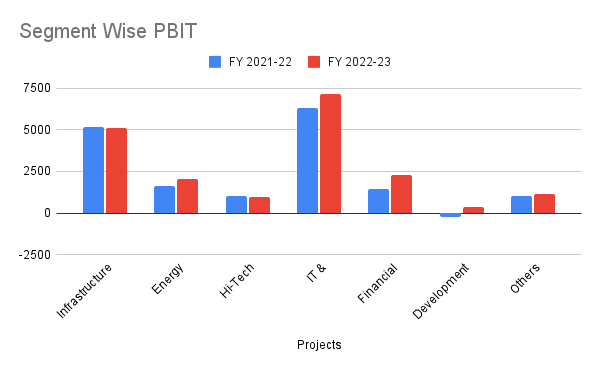
\includegraphics[width=0.8\textwidth]{Segment Wise PBIT.png}
    \caption{Segment Wise PBIT}
  \end{figure}
  

The segment-wise PBIT registered improvement over the
previous year, majorly in Energy Projects, IT\&TS businesses
and Financial Services business. Further, the PBIT of
Development Projects turned positive during the year
primarily due to the value restatement for Nabha Power
Limited (NPL), in line with the improvement in benchmark
valuations due to the visibility of improved profitability and
favourable outcomes of company-specific litigations.

\subsubsection{Other Income}

It mainly consists of profit on the sale of liquid/short-term investments and interest income. Other income at ¢2,929 crore improved by 29.2\% over ¢2,267 crore, reflective of higher investible surpluses and efficient treasury operations.

\subsubsection{Finance Cost}

The interest expense for FY 2022-23 at ¢3,207 crore was marginally higher by 2.6\% over ¢3,126 crore for the previous year. The reduction in average borrowing at a group level was partly offset by an increase in interest rates during the year. Further, refinancing of Hyderabad Metro term loans with market borrowings also contributed to the containment of the interest cost for the year.

\subsubsection{Tax Expense}

The Income Tax charge for FY 2022-23 was higher at ¢4,484 crore by 6.7\% compared to ¢4,204 crore in the previous year on increased profits.

\subsubsection{Exceptional Items}

Exceptional items during the year mainly comprise divestment of the Mutual Fund business of the Financial Services, partially offset by a one-time charge on remeasurement of the wholesale loan assets of the Financial Services segment at fair value. The previous year mainly included divestment gain on the sale of L\&T Uttaranchal Hydropower Limited, partly offset by tax liabilities on the transfer of L\&T-Nxt to the erstwhile Mindtree Limited.

\subsubsection{Consolidated Profit After Tax and EPS}

Consolidated Profit After Tax (PAT) at ¢10,471 crore for FY 2022-23 increased by 20.8\% over the previous year at ¢8,669 crore. The increase is mainly on account of growth in revenues and other income. Consolidated Basic Earnings per Share (EPS) for FY 2022-23 at ¢74.51 improved over the previous year at ¢61.71.

\subsubsection{Return on Consolidated Net Worth}

The Consolidated Net Worth, as at March 31, 2023, at ¢89,326 crore, reflects a net increase of ¢6,918 crore, as compared to the position as at March 31, 2022. The Return on Net Worth (RONW) for FY 2022-23 was higher at 12.2\%, compared to 11.0\% in the previous year, mainly on account of higher profits.

\subsubsection{Liquidity and Gearing}

Cash flow from Operations (including change in loans and advances towards financing activities) increased to ¢22,777 crore as compared to ¢19,163 crore in the previous year, supported by healthy execution and smart working capital management. During the year, additional funds were also generated mainly from the divestment of the Mutual Fund business of the Financial Services business, treasury, and dividend income.

Funds were utilized mainly for repayment of borrowings of ¢4,832 crore, capital expenditure of ¢3,793 crore, and payment of dividend of ¢3,091 crore. Further, funds were applied for the purchase of current investments of ¢8,955 crore and net interest payment of ¢3,047 crore during FY 2022-23.

Consequently, there was a net increase of ¢2,893 crore in the cash balances as at March 31, 2023, compared to the beginning of the financial year.

The total Group borrowings as at March 31, 2023, was lower at ¢118,513 crore, compared to ¢123,468 crore as at March 31, 2022. The major decrease is in borrowings of the Parent entity, Financial Services, and Nabha Power. At a Group level, the gross debt-equity ratio decreased to 1.14:1 as at March 31, 2023, from 1.29:1 as at March 31, 2022. The net debt-equity ratio improved to 0.62:1 as at March 31, 2023, from 0.81:1 as at March 31, 2022.

% \usepackage{tabularray}
\begin{longtblr}[
    caption = {Financial Ratios Comparison},
  ]{
    width = \linewidth,
    colspec = {Q[71]Q[583]Q[90]Q[90]Q[100]},
    column{odd} = {c},
    column{4} = {c},
    hlines,
    vlines,
  }
  \textbf{Sr. No.} & \textbf{Particulars}                                                              & \textbf{FY 21-22} & \textbf{FY 22-23} & \textbf{\% Growth} \\
  (i)              & Gross Debt Equity Ratio                                                           & 1.29              & 1.14              & 11.6\%             \\
  (ii)             & PBDIT as \% of net revenue                                                        & 11.6\%            & 11.3\%            & -2.7\%             \\
  (iii)            & Net Working Capital as \% of Sales (Excluding Financial Services and Corporate)   & 19.7\%            & 16.1\%            & 18.2\%             \\
  (iv)             & Interest Coverage Ratio (excluding Financial Services and Finance Lease Activity) & 5.14              & 5.45              & 6.2\%              
  \end{longtblr}


  \subsection{Strategic Objectives}

\subsubsection{SO-I: Value-accretive growth of current businesses}

\textbf{Performance Measures:}
\begin{itemize}
    \item Revenue growth
    \item Composition of Services in total revenues
\end{itemize}

In FY 2022-23, with a return to normalcy of business activities, the Group achieved revenues of ¢183,341 crore (17\% year-on-year). The Services businesses continued to show strong growth (20\% year-on-year) with a stable percentage share in revenues at 30\% in FY 2022-23.

\subsubsection{SO-II: Scaling-up digital and e-commerce businesses}

\textbf{Performance Measures:}
\begin{itemize}
    \item Growth of digital and e-commerce businesses
\end{itemize}

L\&T Data Center and Cloud Services business has been launched in FY 2022-23 with the commencement of construction of Data Centers in Panvel and Kancheepuram. L\&T-SuFin and L\&T EduTech have been scaled-up further, post their formal launch in FY 2021-22.

\subsubsection{SO-III: Developing business offerings to ride the Energy Transition wave}

\textbf{Performance Measures:}
\begin{itemize}
    \item Size of Green Business
    \item New business or business offering developed
\end{itemize}

The Green Business of L\&T grew to ¢413 billion, which is 37\% of standalone revenues in FY 2022-23 (as compared to 34.7\% in FY 2021-22). The Group also made significant progress in the Green Energy business with the signing of MoUs/agreements (with partners, for the development of Green Hydrogen projects) and setting up a pilot plant for Green Hydrogen production at its Hazira facility.

\subsubsection{SO-IV: Divestment of non-core businesses}

\textbf{Performance Measures:}
\begin{itemize}
    \item Divestment of businesses
\end{itemize}

In FY 2022-23, the Group entered into a Share Purchase Agreement to divest its entire stake in L\&T IDPL (a joint venture having investments in road projects and power transmission assets). The Group continues to actively pursue divestments from other non-core assets and is also exploring various alternatives to derisk the current exposure in Hyderabad Metro.

\subsubsection{SO-V: Enabling business sustainability through a high focus on ESG and Shareholder Value Creation}

\textbf{Performance Measures:}
\begin{itemize}
    \item Metrics linked to ESG performance based on materiality, e.g.,
    \begin{itemize}
        \item Carbon footprint - 29,116 ton CO2 Emissions avoided
        
        \item Resource consumption - 24\%
        Non-Virgin/Recycled and
        eco-friendly materials used
        \item LTIFR (Lost Time Injury Frequency Rate) - 0.06
        LTIFR
        \item Training hours - 6.9 Mn
        Safety training
        man hours
    \end{itemize}
\end{itemize}

\subsection{Sustainability Governance}

The Company conducts materiality assessment (refer to
Materiality Assessment section) to identify and prioritise the
key material topics pertaining to ESG, based on the relative
importance of these topics to the stakeholders and in the
context of L\&T’s business imperatives. The assessment identified
15 important material topics, on the six capitals.
To report sustainability highlights at an overall level, at least
one KPI has been selected for each material topic based on
the importance attached by investors, rating agencies and
regulators and these are given below.

\subsubsection{Environment}

\begin{table}[ht]
    \centering
    \caption{Environment Sustainability Highlights (in various units per ¢ Billion)}
    \begin{tabular}{|l|c|}
    \hline
    \textbf{Sustainability Category} & \textbf{Value} \\
    \hline
    Energy Consumption Intensity & 9,882 GJ/ ¢ Bn \\
    Sourcing from Renewables &  9.6\%\\
    Emissions (GHG Emission Intensity) & 889 tCO2 e/ ¢ Bn \\
    Carbon Sequestration Potential (from Tree Plantation) & 141,300 tCO2 e \\
    Water Consumption Intensity & 10,155 kL/ ¢ Bn \\
    Wastewater Recycling Efficiency & 68\% \\
    Material Management (Recycled and Eco-friendly Material Used) & 24\% \\
    Green Business (Revenue from Green Business) & 37\% \\
    \hline
    \end{tabular}
    \end{table}
    
    % \usepackage{tabularray}

\subsubsection{Social}
\begin{longtblr}[
    caption = {Social Sustainability Highlights},
  ]{
    width = \linewidth,
    colspec = {Q[846]Q[96]},
    column{2} = {c},
    vlines,
    hline{1-2,12} = {-}{},
  }
  \textbf{Sustainability Category}                                                  & \textbf{Value} \\
  Health and Safety (Safety Training Man Hours)                                     & 6.9 Mn         \\
  Health and Safety (LTIFR1)                                                        & 0.06           \\
  Human Rights (Own Locations Assessed and Complied with Human Rights Requirements) & 100\%          \\
  Workforce Skilling and Talent Management (Employees)                              & 28,000+        \\
  Workforce Skilling and Talent Management (Workers Trained on Skill Upgradation)   & 45,000+        \\
  Workforce Skilling and Talent Management (Attrition Rate)                         & 13.9\%         \\
  Diversity and Inclusion (Diversity)                                               & 7.1\%          \\
  Diversity and Inclusion (Women in Senior Management)                              & 89             \\
  Social Impact (CSR Beneficiaries)                                                 & 1.5 Mn         \\
  Social Impact (MSME Suppliers)                                                    & 10,736         
  \end{longtblr}

\subsubsection{Governance}
    % \usepackage{color}
% \usepackage{tabularray}
\begin{longtblr}[
    caption = {Governance and Ethics Sustainability Highlights},
  ]{
    width = \linewidth,
    colspec = {Q[867]Q[75]},
    cell{1}{2} = {c},
    cell{2}{2} = {c},
    cell{3}{2} = {c},
    cell{4}{2} = {c},
    cell{5}{2} = {c},
    cell{6}{2} = {c},
    cell{7}{2} = {c},
    cell{8}{2} = {c},
    vlines,
    hline{1-2,8-10} = {-}{},
  }
  \textbf{Sustainability Category}                                                             & \textbf{Value} \\
  Governance  Ethics (New Joinees Trained on CoC)                                              & 100\%          \\
  Customer Centricity (Customer Satisfaction Score out of 10)                                  & 9.2            \\
  Data Privacy  Cyber Security                                                                 & 0              \\
  Sustainable Supply Chain (Sustainable Sourcing of Input Material from Neighboring Districts) & 40\%           \\
  Sustainable Supply Chain (Sustainable Value of Input Material Sourced from Suppliers)        & 7\%            \\
  Brand Management (Ranked among 'World's Top 200 Environmental Firms' by ENR for 2022)        & 3rd            \\
  Brand Management (Certified as Great Place To Work®)                                         &                \\
  New Policies (Anti Bribery and Anti Corruption, Equal Opportunity, Public Policy Advocacy)   &                
  \end{longtblr}

\subsection{Long-term commitment }

\subsubsection{NATURAL CAPITAL}
\begin{itemize}
  \item Water consumption: 11 Mn kL
  \item Energy from Non-Renewable sources: 10.61 Mn GJ 
  \item Energy from Renewable sources: 0.13 Mn GJ
  \item Spend on Environment: \$288.4 Mn 
  \item Material consumed \(Mn tonnes\):
    \begin{itemize}
      \item Cement: 4.61 
      \item Sand: 6.95 
      \item Ferrous: 3.06
    \end{itemize}
\end{itemize}

\subsubsection{MANUFACTURED CAPITAL}
\begin{itemize}
  \item Active Project Sites: 729 
  \item Manufacturing plants: 18
\end{itemize}

\subsubsection{SOCIAL AND RELATIONSHIP CAPITAL}
\begin{itemize}
  \item CSR spend: ¢ 1.4 Bn 
  \item CSR partners: 64
  \item MSME suppliers: 10,736
  \item Memberships of Industry Chambers: 75
\end{itemize}

\subsubsection{HUMAN CAPITAL}
\begin{itemize}
  \item Employees: 55,202
  \item Engineers: 41,000 
  \item Workmen: 277,857 
  \item Employees covered under Leadership Development Programmes: 1,672
\end{itemize}

\subsubsection{FINANCIAL CAPITAL}
\begin{itemize}
  \item Order Book: \$3,305.5 Bn
  \item Net Current Assets: \$324.9 Bn 
  \item Net Fixed Assets: \$117.1 Bn
\end{itemize}

\subsubsection{INTELLECTUAL CAPITAL}
\begin{itemize}
  \item R\&D spend (cumulative last 3 years): \$3,448 Mn 
  \item Patents filed: 8
  \item R\&D Engineers and Scientists: 380
  \item Active collaborations and partnerships: 20
\end{itemize}


